\documentclass{article}

\usepackage{lipsum}
\usepackage{amsfonts}
\usepackage{amsmath}
\usepackage{amsthm}
\usepackage{graphicx}
\graphicspath{{figures/5_18_22/}}
\usepackage{epstopdf}
\ifpdf%
\DeclareGraphicsExtensions{.eps,.pdf,.png,.jpg}
\else
\DeclareGraphicsExtensions{.eps}
\fi
\usepackage{amsopn}
\DeclareMathOperator{\diag}{diag}
\usepackage{booktabs}
\usepackage{bbm}
\usepackage{bm}
\usepackage{caption}
\usepackage{subcaption}
\usepackage[utf8]{inputenc}
\usepackage[T1]{fontenc}
\usepackage[margin=1in]{geometry}
\usepackage{hyperref}
\usepackage{algorithm}
\usepackage{algpseudocode}
\usepackage{placeins}
\usepackage{cleveref}

\newcommand{\norm}[1]{\left\lVert#1\right\rVert}
\newcommand{\normtwo}[1]{\left\lVert#1\right\rVert_2}
\newcommand{\abs}[1]{\left\lvert#1\right\rvert}
\newcommand{\mat}[1]{\bm{{#1}}}
\renewcommand{\vec}[1]{\bm{{#1}}}
\newcommand{\lequiv}{\Leftrightarrow}
\newcommand{\bigO}[1]{\mathcal{O}\!\left(#1\right)}
\newcommand{\ceil}[1]{\left\lceil #1 \right\rceil}
\newcommand{\floor}[1]{\left\lfloor #1 \right\rfloor}
\newcommand{\sfrac}[2]{#1/#2}
\newcommand{\hquad}{\enskip}
\newcommand{\expected}[1]{\mathbb{E}\left[#1\right]}
\newcommand{\mspan}[1]{\text{span}\left( #1 \right)}
\newcommand{\prob}[1]{P\left(#1\right)}
\newcommand{\probt}[1]{P\left( \text{#1} \right)}
\newcommand{\condprob}[2]{P\left(#1 \:|\: #2\right)}
\newcommand{\condprobt}[2]{P\left(\text{#1} \:|\: \text{#2}\right)}
\newcommand{\bayes}[2]{\frac{\condprob{#2}{#1}\prob{#1}}{\prob{#2}}}
\newcommand{\bayesx}[3]{\frac{\condprob{#2}{#1}\prob{#1}}{\condprob{#2}{#1}\prob{#1} + \condprob{#2}{#3}\prob{#3}}}
\newcommand{\sech}{\text{sech}}
\newcommand*{\vertbar}{\rule[-1ex]{0.5pt}{2.5ex}}
\newcommand*{\horzbar}{\rule[.5ex]{2.5ex}{0.5pt}}
\newcommand{\vect}[2]{\underline{{#1}}_{{#2}}}
\newcommand{\basisp}[1]{\underline{{p}}_{{#1}}}
\newcommand{\basisq}[1]{\underline{{q}}_{{#1}}}
\newcommand{\coeff}[1]{\underline{{a}}_{{#1}}}
\newcommand{\bestfit}{\underline{\bar{x}}}
\newcommand{\grad}{\nabla}
\newcommand{\laplace}{\Delta}
\newcommand{\setbar}{\:\middle|\:}
\renewcommand{\div}{\grad \cdot}
\renewcommand{\Re}{\text{Re}}
\newcommand{\var}[1]{\texttt{{#1}}}

\begin{document}
%% \section{Background}

Learning aggregation for 3D anisotropic diffusion on a structured grid
\begin{equation}
  -\grad \cdot \left(\mat{D} \grad u\right) = 0,
\end{equation}
\begin{equation}
  \mat{D} := \mat{R}^T\begin{bmatrix}\varepsilon_x & & \\ & \varepsilon_y & \\ & & 1 \end{bmatrix}\mat{R},
\end{equation}
\begin{equation}
  \mat{R} := \begin{bmatrix} \cos \theta_z & -\sin \theta_z & 0 \\ \sin \theta_z & \cos \theta_z & 0 \\ 0 & 0 & 1\end{bmatrix} \begin{bmatrix}\cos \theta_y & 0 & \sin \theta_y \\ 0 & 1 & 0 \\ -\sin\theta_y & 0 & \cos\theta_y \end{bmatrix}.
\end{equation}

For both the \textit{isotropic} and \textit{anisotropic} cases we generate two sets each of:
\begin{itemize}
\item 500 training problems, and
\item 250 testing problems
\end{itemize}
to train the ML method.  For the anisotropic case, these problems randomly have the parameters $N_x=N_y=N_z=N \sim \mathcal{U}\left\{8, 14\right\}$; $\theta_z, \theta_y \sim \mathcal{U}\left(0, 2\pi\right)$; $\log_{10}\varepsilon_x, \log_{10}\varepsilon_y \sim \mathcal{U}\left(-4, 4\right)$.  The isotropic problems have the same parameter distribution for $N$, while $\theta_z=\theta_y=0$ and $\varepsilon_x=\varepsilon_y=1$.

Each problem was discretized in Firedrake \cite{Firedrake} using piecewise linear tetrahedral finite elements with homogeneous Dirichlet boundary conditions.  Afterwards, the degrees-of-freedom corresponding to Dirichlet boundary conditions were removed from the system.

The network was then trained on the anisotropic problems with a coarsening ratio of $\alpha=0.09=\left(0.1\right)^2$.  In reality, this should be probably around $\alpha=0.027=\left(0.1\right)^3$, but I forgot to set it.  This probably explains why the 2D network gives decent results for the 3D problems: the coarsening ratio was kept constant.

Existing results for the 2D diffusion problems are shown in \cref{tab:conv_2d} for comparison purposes.  Results for the untrained (existing 2D model) and trained (specifically on 3D) networks are given in \cref{tab:conv_3d}.

\begin{table}[h]
  \centering
  \begin{tabular}{c c c c c c c}
    \textbf{Problem Type} & \textbf{Data Set} & \textbf{Random Conv.} & \textbf{Lloyd Conv.} & \textbf{Full ML Conv.} & \textbf{ML Agg.} & \textbf{ML Int.} \\
    \hline
    Isotropic & Train & 0.4652 & 0.4208 & 0.3956 & 0.3974 & 0.4190 \\
    Isotropic & Test & 0.4623 & 0.4177 & 0.3913 & 0.3922 & 0.4172 \\
    Anisotropic & Train & 0.7680 & 0.7705 & 0.7462 & 0.7532 & 0.7614 \\
    Anisotropic & Test & 0.7902 & 0.7978 & 0.7727 & 0.7776 & 0.7910 \\
    \hline
  \end{tabular}
  \caption{Existing results for the 2D diffusion problems.  This model has been trained on both isotropic and anisotropic diffusion in 2D.  The column for \textit{Full ML Conv.} is the method that uses the model for both aggregation and smoothing.  \textit{ML Agg.} and \textit{ML Int.} refer to ML aggregation and Jacobi smoothing, Lloyd aggregation and ML smoothing, respectively.}
  \label{tab:conv_2d}
\end{table}

\begin{table}[h]
  \centering
  \begin{tabular}{c c c c c}
    \textbf{Model} & \textbf{Data Set} & \textbf{Random Conv.} & \textbf{Lloyd Conv.} & \textbf{ML Conv.} \\
    \hline
    Untrained & Iso., Train & 0.3699 & 0.3933 & 0.3362 \\
    Untrained & Iso., Test & 0.3697 & 0.3874 & 0.3243 \\
    \hline
    Untrained & Aniso., Train & 0.7064 & 0.7117 & 0.7153 \\
    Untrained & Aniso., Test & 0.7073 & 0.7133 & 0.7241 \\
    \hline
    \hline
    Trained & Iso., Train & 0.3699 & 0.3933 & 0.3364 \\
    Trained & Iso., Test & 0.3697 & 0.3874 & 0.3330 \\
    \hline
    Trained & Aniso., Train & 0.7064 & 0.7117 & 0.7107 \\
    Trained & Aniso., Test & 0.7073 & 0.7133 & 0.7196 \\
    \hline
  \end{tabular}
  \caption{Convergence of ML vs baseline, Lloyd methods on training, testing 3D datasets. \textit{Trained} refers to the model trained specifically on the 3D diffusion problems while \textit{untrained} is the existing 2D model (see \cref{tab:conv_2d}).}
  \label{tab:conv_3d}
\end{table}

\begin{figure}[!hb]
  \centering
  \begin{subfigure}[t]{0.49\textwidth}
    \centering
    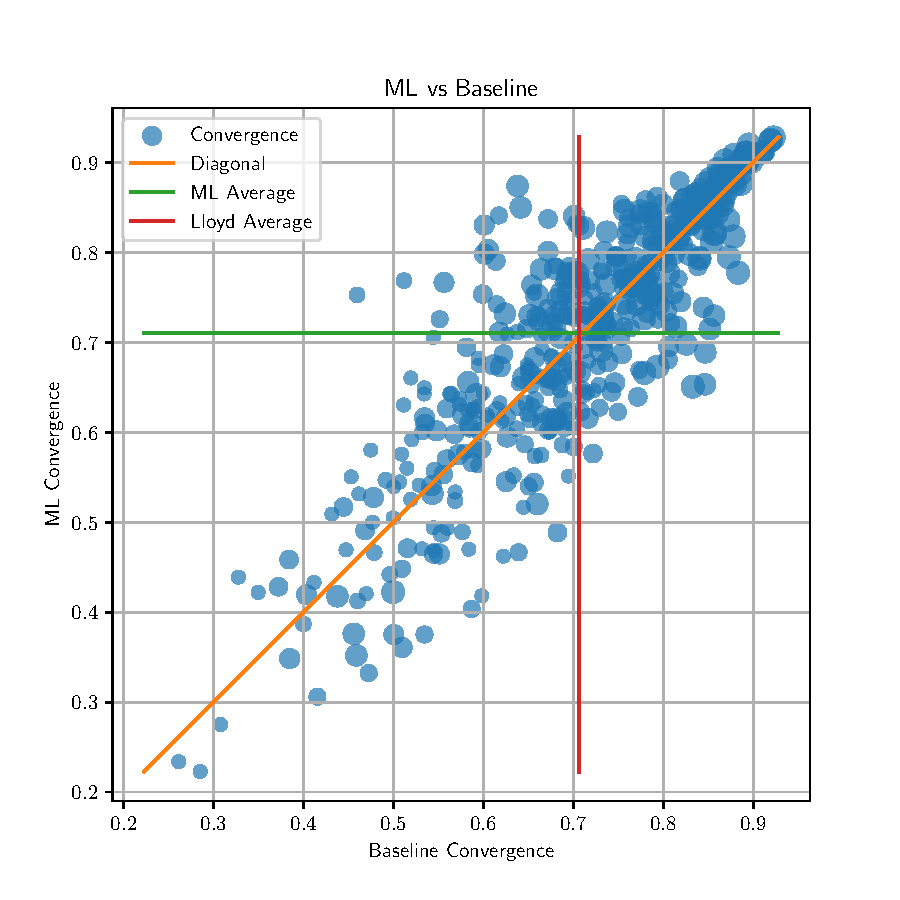
\includegraphics[width=\textwidth]{aniso3d_train_baseline_ml_convergence.pdf}
    \caption{Training convergence}
  \end{subfigure}
  \begin{subfigure}[t]{0.49\textwidth}
    \centering
    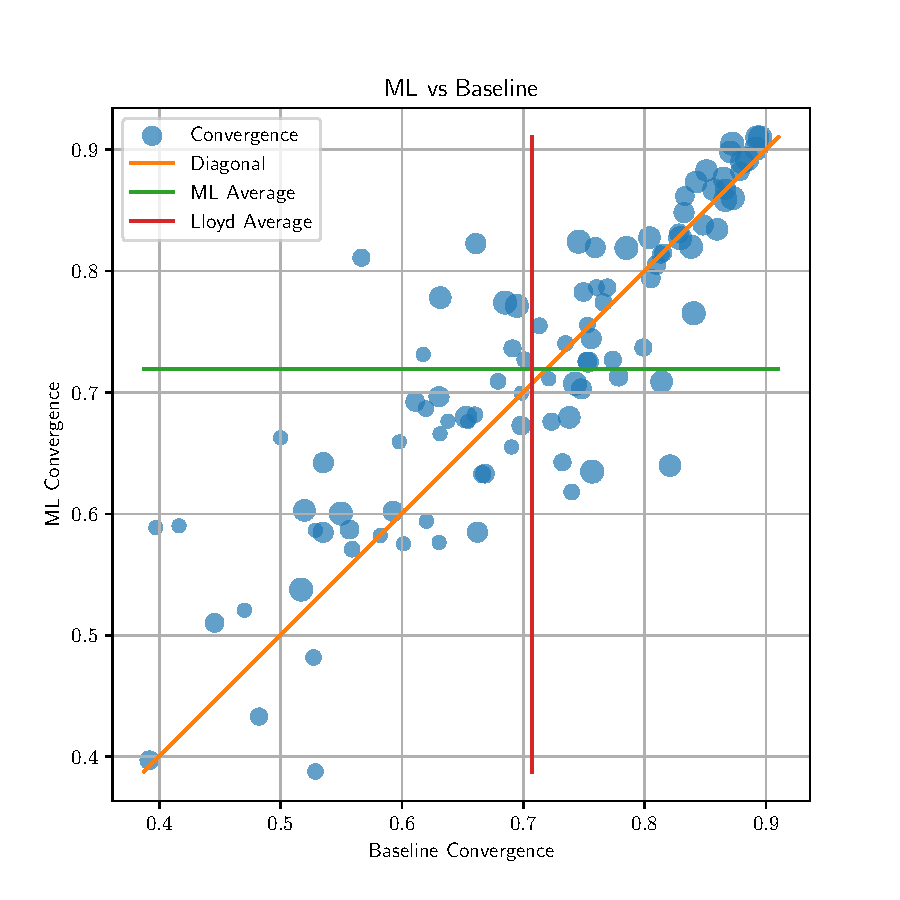
\includegraphics[width=\textwidth]{aniso3d_test_baseline_ml_convergence.pdf}
    \caption{Testing convergence}
  \end{subfigure}
  \caption{Convergence data for the ML AMG method vs a Lloyd and Jacobi SA method on the anisotropic datasets.  Values below the diagonal indicate a better convergence for the ML.  Markers are scaled by problem size.}
  \label{fig:aniso_conv}
\end{figure}
\bigskip\bigskip
\begin{figure}[!htb]
  \centering
  \begin{subfigure}[t]{0.49\textwidth}
    \centering
    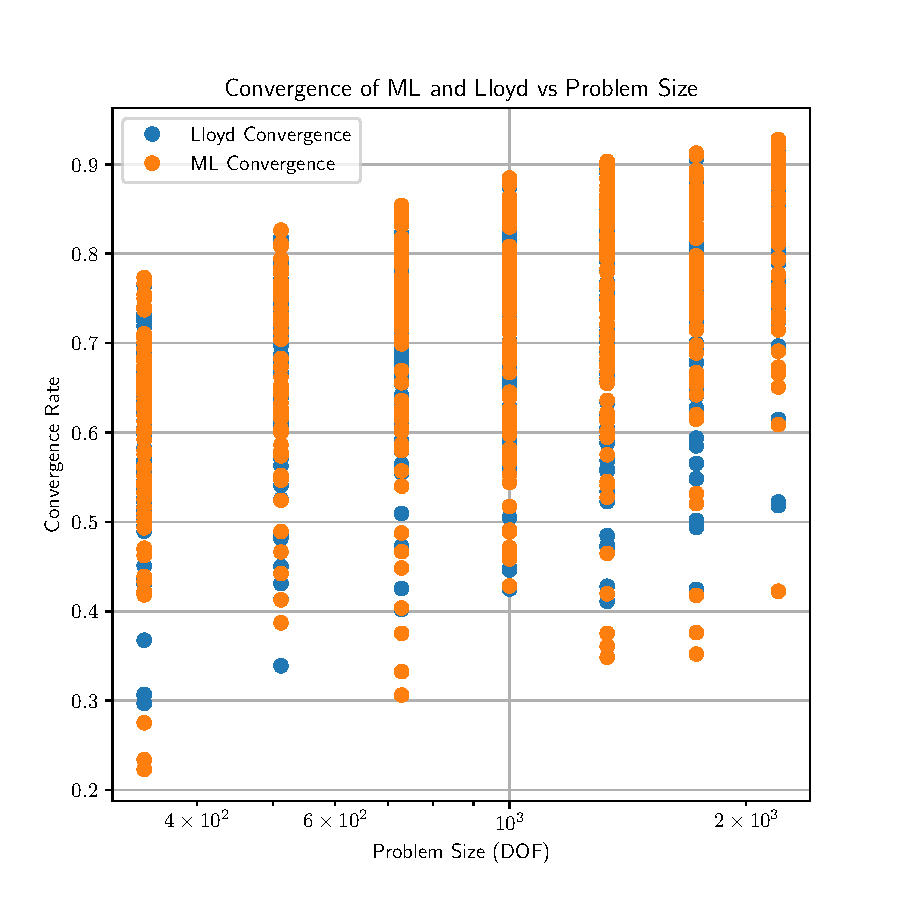
\includegraphics[width=\textwidth]{aniso3d_train_convergence_per_size.pdf}
    \caption{Training convergence}
  \end{subfigure}
  \begin{subfigure}[t]{0.49\textwidth}
    \centering
    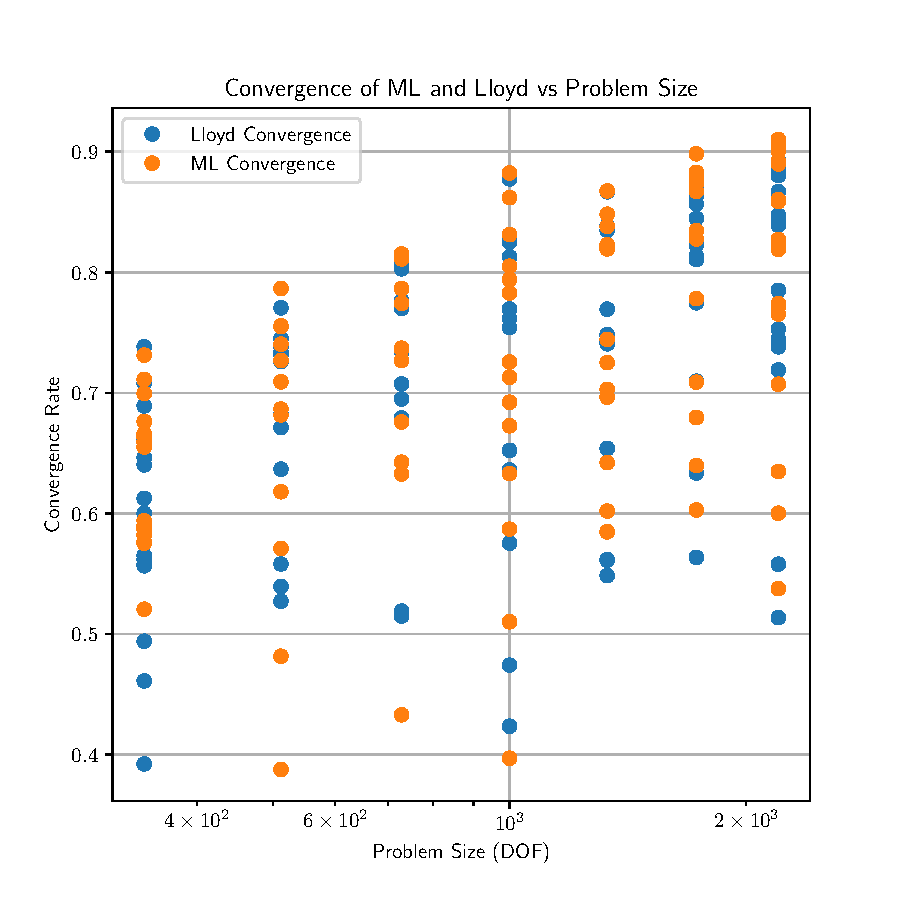
\includegraphics[width=\textwidth]{aniso3d_test_convergence_per_size.pdf}
    \caption{Testing convergence}
  \end{subfigure}
  \caption{Convergence data for the two methods plotted against problem size (DOF) for anisotropic datasets.}
  \label{fig:aniso_conv_per_size}
\end{figure}

\begin{figure}[h!]
  \centering
  \begin{subfigure}[t]{0.49\textwidth}
    \centering
    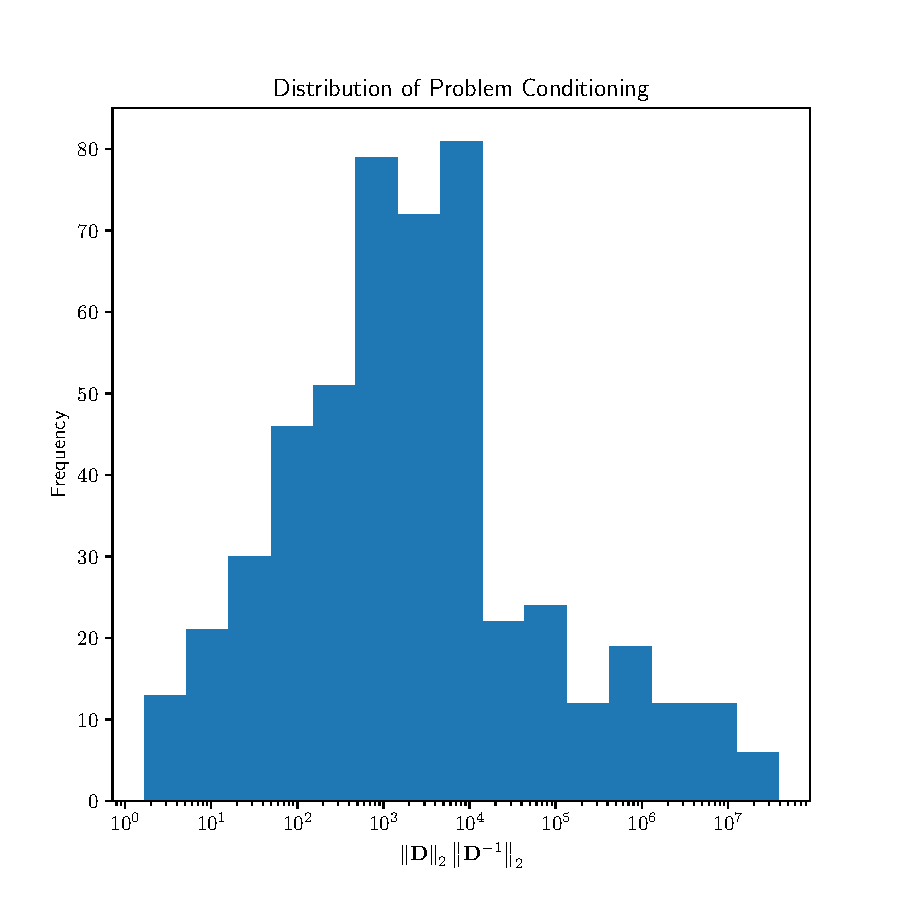
\includegraphics[width=\textwidth]{aniso3d_train_cond_hist.pdf}
    \caption{Training Conditioning}
  \end{subfigure}
  \begin{subfigure}[t]{0.49\textwidth}
    \centering
    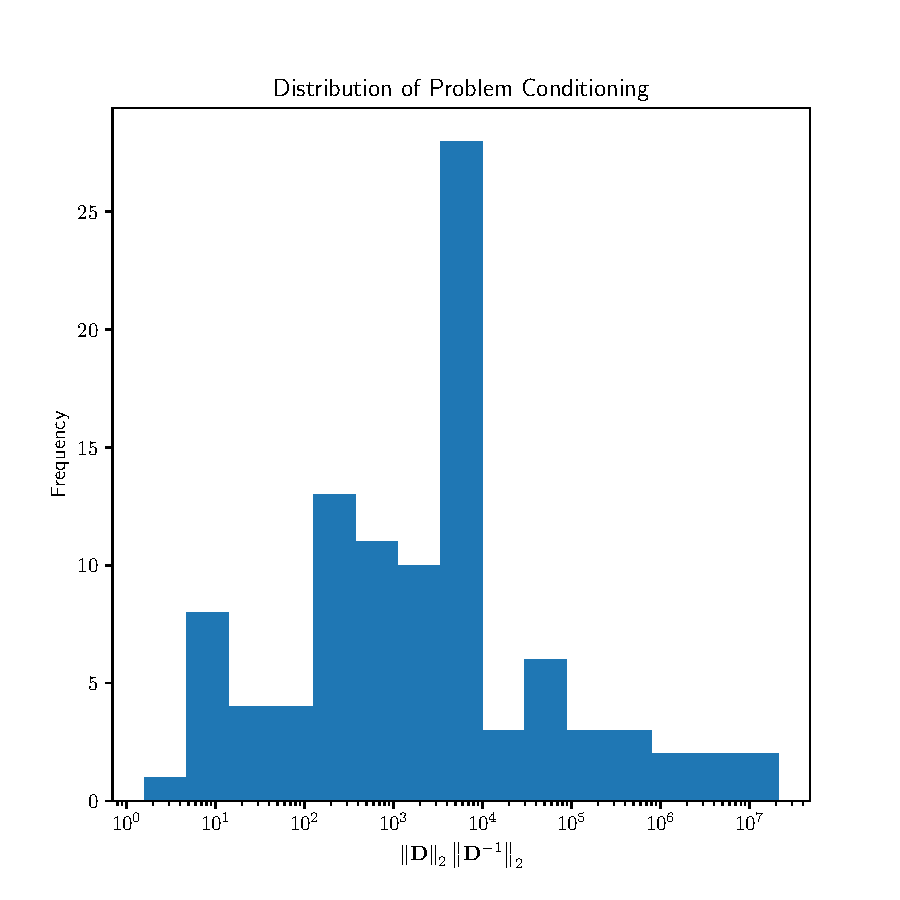
\includegraphics[width=\textwidth]{aniso3d_test_cond_hist.pdf}
    \caption{Testing Conditioning}
  \end{subfigure}
  \caption{Histograms of problem conditioning for both anisotropic training and testing datasets.}
  \label{fig:cond_hist}
\end{figure}

\begin{figure}[h!]
  \centering
  \begin{subfigure}[t]{0.49\textwidth}
    \centering
    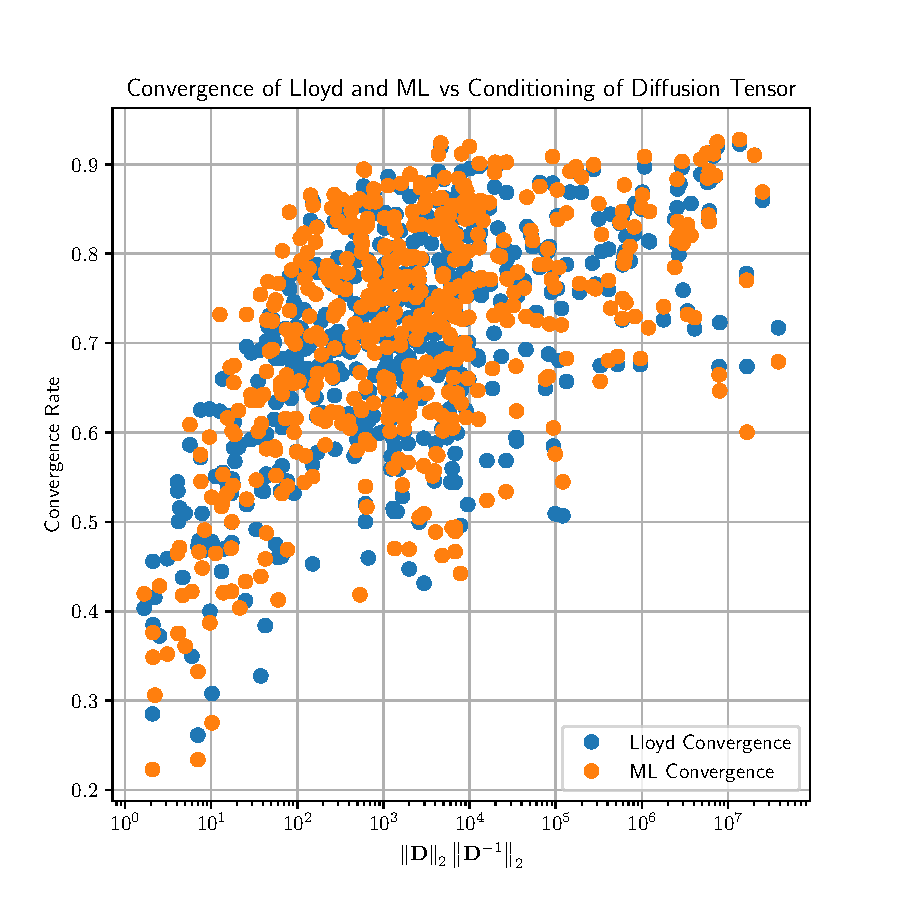
\includegraphics[width=\textwidth]{aniso3d_train_convergence_per_cond.pdf}
    \caption{Training Convergence}
  \end{subfigure}
  \begin{subfigure}[t]{0.49\textwidth}
    \centering
    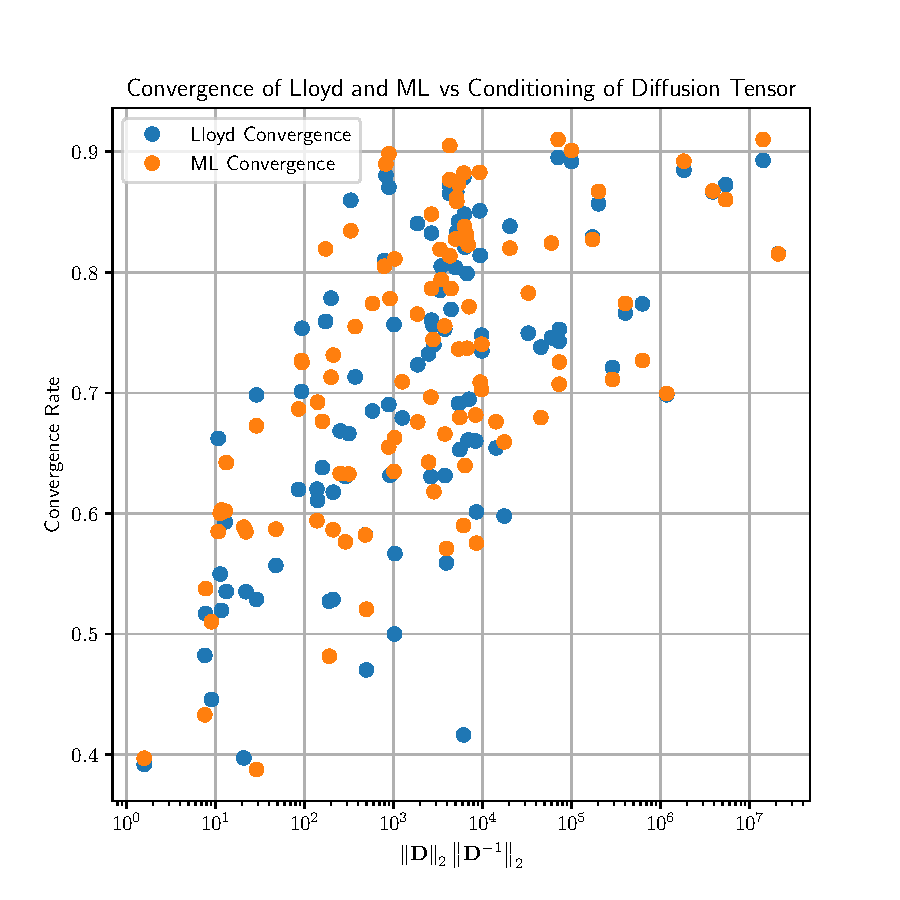
\includegraphics[width=\textwidth]{aniso3d_test_convergence_per_cond.pdf}
    \caption{Testing Convergence}
  \end{subfigure}
  \caption{Convergence on both anisotropic datasets per ratio of extremal eigenvalues of the diffusion tensor.}
  \label{fig:aniso_conv_per_eps}
\end{figure}

\begin{figure}[h!]
  \centering
  \begin{subfigure}[t]{0.47\textwidth}
    \centering
    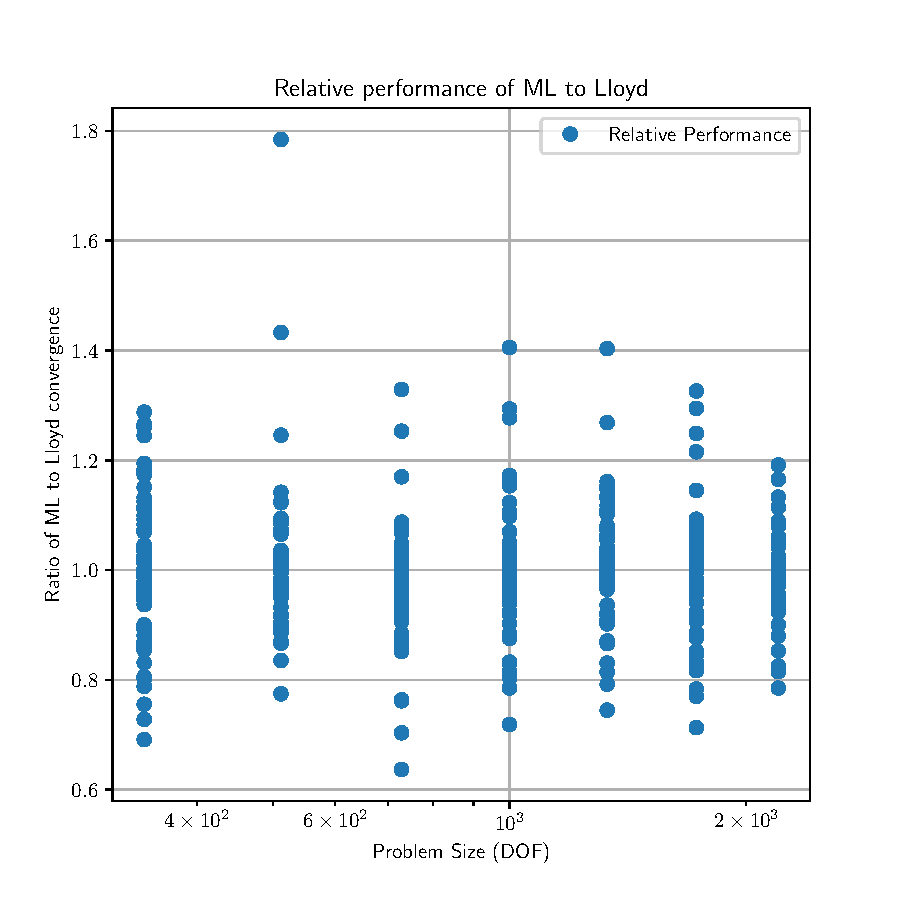
\includegraphics[width=\textwidth]{aniso3d_train_rel_perf.pdf}
    \caption{Relative training performance}
  \end{subfigure}
  \begin{subfigure}[t]{0.47\textwidth}
    \centering
    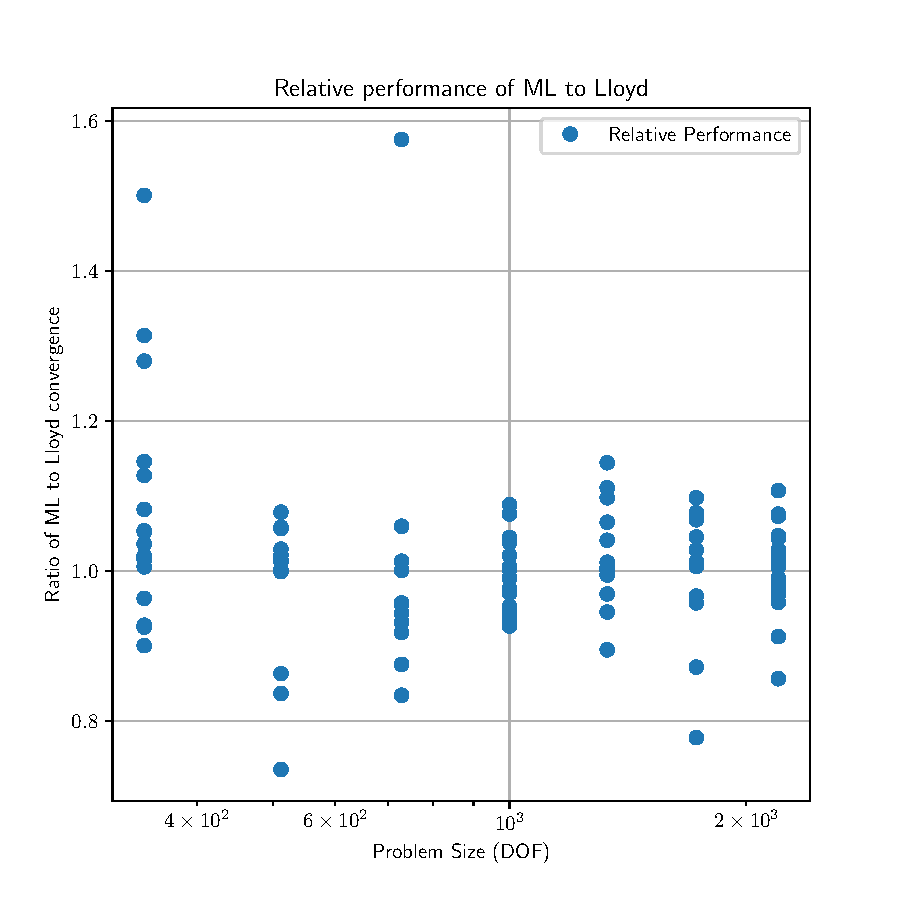
\includegraphics[width=\textwidth]{aniso3d_test_rel_perf.pdf}
    \caption{Relative testing performance}
  \end{subfigure}
  \caption{Relative performance of the ML to the Lloyd method, plotted against problem size for the anisotropic datasets.  Relative performance is obtained by dividing the ML convergence by the Lloyd convergence for each problem.  Values below $1$ indicate better ML performance, while values above $1$ indicate better baseline performance.}
  \label{fig:aniso_rel_conv}
\end{figure}

\bibliographystyle{siam}
\bibliography{navier}
\end{document}
